% !TEX root = ../Report.tex
\appendix

\chapter{Evaluation Day Survey Instrument and Results}
\label{appx:survey}

This appendix contains supporting evidence from the Evaluation Day survey. The
main body of the report presents the key findings; the complete survey export is
included here to allow assessors to inspect the full distribution of responses.

\section{Survey Questions (Summary)}
The survey included:
\begin{itemize}
  \item Git familiarity and feature usage questions,
  \item System Usability Scale (SUS) items,
  \item Git concept understanding Likert items,
  \item Core functionality Likert items,
  \item Overall impression Likert items,
  \item free-text questions on positives, frustrations, adoption likelihood,
        and comparison to current workflows.
\end{itemize}

\section{Full Survey Export PDF}
\textbf{Compilation note:} place \texttt{eval\_day\_survey\_results.pdf} in the
same directory as this \texttt{.tex} file, or update the path below.

% Uncomment the line below once the PDF is available:
% \includepdf[pages=-]{Appendices/eval_day_survey_results.pdf}

\chapter{User Acceptance Test Results (Full Tables)}
\label{appx:uat}

This appendix reproduces the full UAT results from Evaluation Day for archival
completeness. Summary statistics are presented in Chapter~8; the raw data is
included here to allow detailed inspection.

\begin{table}[H]
\centering
\caption{UAT Task T1 --- Auto-schedule feasibility (full results).}
\begin{tabular}{@{}lcccc@{}}
\toprule
\textbf{Participant} & \textbf{Completed?} & \textbf{Time} &
\textbf{Non-overlapping?} & \textbf{Non-zero travel gaps?} \\
\midrule
P1  & Y & 3:12  & Y & Y \\
P2  & Y & 4:45  & Y & Y \\
P3  & Y & 2:58  & Y & Y \\
P4  & Y & 5:30  & Y & Y \\
P5  & Y & 3:44  & Y & Y \\
P6  & Y & 6:02  & Y & Y \\
P7  & N & 8:00* & -- & -- \\
P8  & Y & 4:11  & Y & Y \\
P9  & Y & 3:55  & Y & Y \\
P10 & Y & 4:28  & Y & Y \\
\bottomrule
\end{tabular}

\vspace{0.3em}
{\footnotesize *P7 timed out due to difficulty locating the auto-scheduler
button without a hint.}
\end{table}

\begin{table}[H]
\centering
\caption{UAT Task T2 --- Merge conflict resolution (full results).}
\begin{tabular}{@{}lccc@{}}
\toprule
\textbf{Participant} & \textbf{Resolved?} & \textbf{Time} &
\textbf{Hints given} \\
\midrule
P1  & Y & 2:34  & 0 \\
P2  & Y & 4:50  & 1 \\
P3  & Y & 1:58  & 0 \\
P4  & Y & 3:22  & 0 \\
P5  & Y & 4:47  & 1 \\
P6  & N & 6:10* & 2 \\
P7  & Y & 3:05  & 1 \\
P8  & Y & 2:41  & 0 \\
P9  & Y & 4:33  & 1 \\
P10 & Y & 3:18  & 0 \\
\bottomrule
\end{tabular}

\vspace{0.3em}
{\footnotesize *P6 selected the wrong branch and ran out of time.}
\end{table}

\begin{table}[H]
\centering
\caption{UAT Task T3 --- Quick edit and save without Git explanation (full
results).}
\begin{tabular}{@{}lcp{0.55\linewidth}@{}}
\toprule
\textbf{Participant} & \textbf{Completed?} & \textbf{Notes} \\
\midrule
P1  & Y & Edited timeline stop duration naturally \\
P2  & Y & Used ``Save'' without prompting \\
P3  & Y & -- \\
P4  & N & Asked ``does saving here create a version?'' \\
P5  & Y & -- \\
P6  & Y & -- \\
P7  & Y & -- \\
P8  & N & Hesitated; unsure if edit was auto-saved \\
P9  & Y & -- \\
P10 & Y & -- \\
\bottomrule
\end{tabular}
\end{table}

\chapter{Additional Diagrams and Screenshots}
\label{appx:diagrams}

% TODO: Replace each placeholder below with a real screenshot.
%       Save screenshots as PNG/PDF in the Appendices/ folder and use:
%       \includegraphics[width=0.92\linewidth]{Appendices/filename.png}

\begin{figure}[H]
  \centering
  % 
\includegraphics[width=0.92\linewidth]{Appendices/merge-ui.png}
  \fbox{\parbox{0.92\linewidth}{\centering TODO: screenshot of the merge
  conflict resolution UI showing ours/theirs choices and the resolve button.}}
  \caption{Merge conflict resolution UI.}
\end{figure}

\begin{figure}[H]
  \centering
  % \includegraphics[width=0.92\linewidth]{Appendices/timeline-editor.png}
  \fbox{\parbox{0.92\linewidth}{\centering TODO: screenshot of the timeline
  editor with draggable stop blocks showing arrival/departure times.}}
  \caption{Timeline editor with draggable stop blocks.}
\end{figure}

\begin{figure}[H]
  \centering
  % \includegraphics[width=0.92\linewidth]{Appendices/map-editor.png}
  \fbox{\parbox{0.92\linewidth}{\centering TODO: screenshot of the map editor
  showing numbered markers, route polylines, and transit leg styling.}}
  \caption{Map editor with numbered markers and route geometry.}
\end{figure}

\begin{figure}[H]
  \centering
  % \includegraphics[width=0.92\linewidth]{Appendices/easy-mode.png}
  \fbox{\parbox{0.92\linewidth}{\centering TODO: screenshot comparing Easy mode
  (simplified controls) vs Git mode (branches, commits, merge visible).}}
  \caption{Easy mode vs Git mode comparison.}
\end{figure}

\begin{figure}[H]
  \centering
  % \includegraphics[width=0.92\linewidth]{Appendices/algo-visualisation.png}
  \fbox{\parbox{0.92\linewidth}{\centering TODO: screenshot of the algorithm
  visualisation page showing the map, pseudocode highlighting, and playback
  controls.}}
  \caption{Algorithm visualisation page.}
\end{figure}

\begin{figure}[H]
  \centering
  % \includegraphics[width=0.92\linewidth]{Appendices/quick-explore.png}
  \fbox{\parbox{0.92\linewidth}{\centering TODO: screenshot of the quick
  explore mode showing the optimised route with summary stats.}}
  \caption{Quick explore mode with optimised route.}
\end{figure}

\chapter{Project Schedule}
\label{appx:schedule}

Figure~\ref{fig:gantt} shows the project timeline across the two terms of the
2025/26 academic year. Table~\ref{tab:schedule_detail} provides a breakdown of
deliverables per phase.

\begin{figure}[H]
  \centering
  \resizebox{\textwidth}{!}{%
  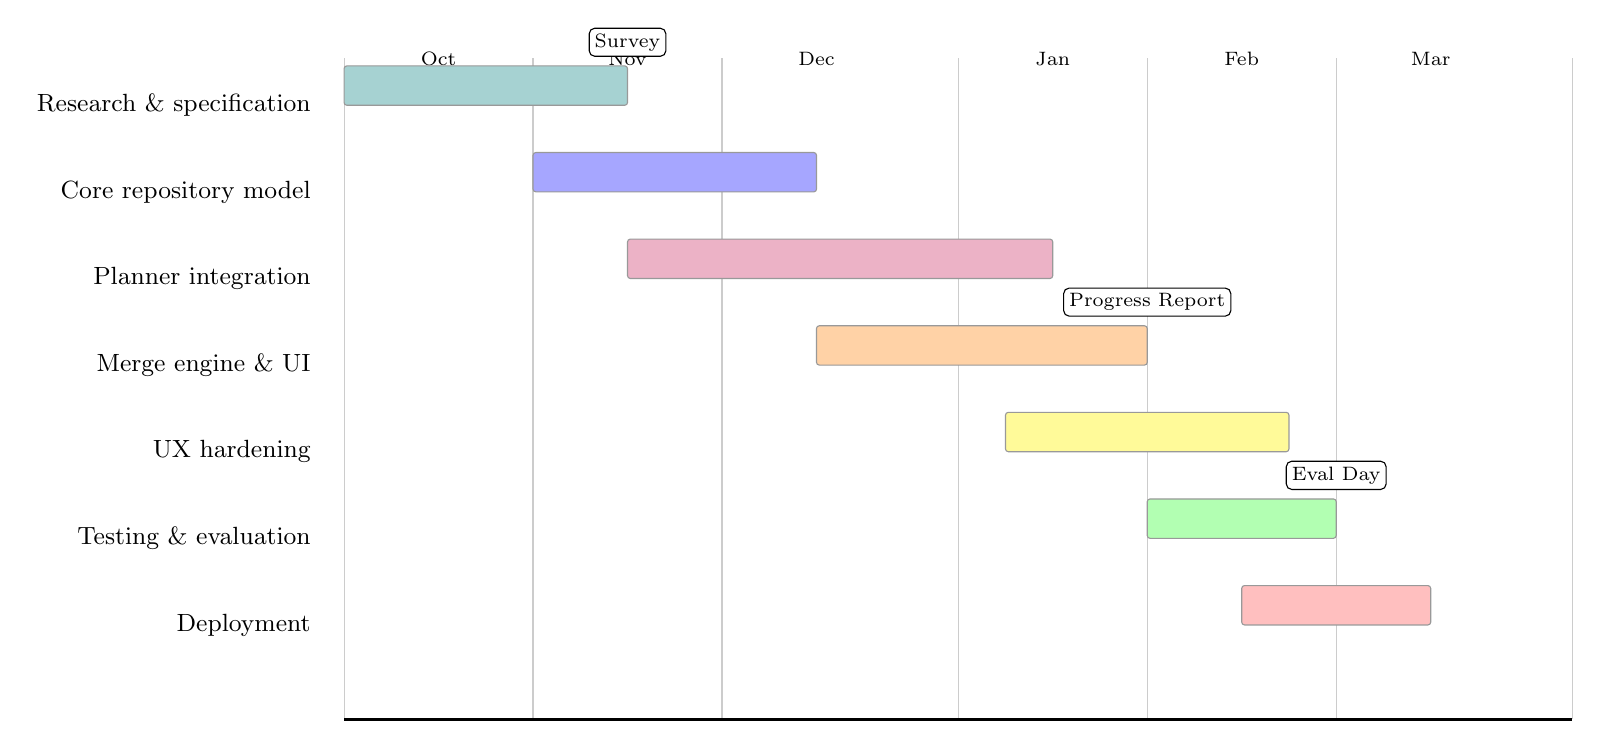
\begin{tikzpicture}[
    every node/.style={font=\small},
    bar/.style={fill=#1, draw=black!40, rounded corners=1pt, minimum height=0.5cm},
    bar/.default={blue!30},
    phaselabel/.style={font=\small, anchor=east},
    monthlabel/.style={font=\scriptsize, anchor=north},
  ]
    % Time axis: Oct 2025 to Mar 2026 = 6 months, 1cm per week (26 weeks)
    % Oct=4w, Nov=4w, Dec=4w, Jan=5w, Feb=4w, Mar=5w (approx)
    \def\wk{0.6}  % cm per week

    % Month boundaries (cumulative weeks)
    \def\octStart{0}
    \def\novStart{4}
    \def\decStart{8}
    \def\janStart{13}
    \def\febStart{17}
    \def\marStart{21}
    \def\totalWk{26}

    % Grid lines
    \foreach \m/\lbl in {\octStart/Oct,\novStart/Nov,\decStart/Dec,\janStart/Jan,\febStart/Feb,\marStart/Mar} {
      \draw[black!20] (\m*\wk, 0.6) -- (\m*\wk, -7.8);
      \node[monthlabel] at (\m*\wk + 2*\wk, 0.8) {\lbl};
    }
    \draw[black!20] (\totalWk*\wk, 0.6) -- (\totalWk*\wk, -7.8);

    % Phase bars (y positions)
    \def\yA{0}
    \def\yB{-1.1}
    \def\yC{-2.2}
    \def\yD{-3.3}
    \def\yE{-4.4}
    \def\yF{-5.5}
    \def\yG{-6.6}

    % Labels
    \node[phaselabel] at (-0.3, \yA) {Research \& specification};
    \node[phaselabel] at (-0.3, \yB) {Core repository model};
    \node[phaselabel] at (-0.3, \yC) {Planner integration};
    \node[phaselabel] at (-0.3, \yD) {Merge engine \& UI};
    \node[phaselabel] at (-0.3, \yE) {UX hardening};
    \node[phaselabel] at (-0.3, \yF) {Testing \& evaluation};
    \node[phaselabel] at (-0.3, \yG) {Deployment};

    % Bars: (start week * wk, y) rectangle (end week * wk, y + 0.5)
    % Research: Oct wk1 - Nov wk2 (weeks 0-6)
    \fill[bar=teal!35] (0*\wk, \yA) rectangle (6*\wk, \yA+0.5);
    % Core repo: Nov wk1 - Dec wk2 (weeks 4-10)
    \fill[bar=blue!35] (4*\wk, \yB) rectangle (10*\wk, \yB+0.5);
    % Planner: Nov wk3 - Jan wk2 (weeks 6-15)
    \fill[bar=purple!30] (6*\wk, \yC) rectangle (15*\wk, \yC+0.5);
    % Merge: Dec wk2 - Jan wk4 (weeks 10-17)
    \fill[bar=orange!35] (10*\wk, \yD) rectangle (17*\wk, \yD+0.5);
    % UX: Jan wk2 - Feb wk3 (weeks 14-20)
    \fill[bar=yellow!40] (14*\wk, \yE) rectangle (20*\wk, \yE+0.5);
    % Testing: Jan wk4 - Feb wk4 (weeks 17-21)
    \fill[bar=green!30] (17*\wk, \yF) rectangle (21*\wk, \yF+0.5);
    % Deployment: Feb wk2 - Mar wk2 (weeks 19-23)
    \fill[bar=red!25] (19*\wk, \yG) rectangle (23*\wk, \yG+0.5);

    % Milestone markers
    \node[font=\scriptsize, fill=white, draw=black, rounded corners=2pt,
          inner sep=2pt] at (6*\wk, \yA+0.5+0.3) {Survey};
    \node[font=\scriptsize, fill=white, draw=black, rounded corners=2pt,
          inner sep=2pt] at (17*\wk, \yD+0.5+0.3) {Progress Report};
    \node[font=\scriptsize, fill=white, draw=black, rounded corners=2pt,
          inner sep=2pt] at (21*\wk, \yF+0.5+0.3) {Eval Day};

    % Bottom axis
    \draw[thick] (0, -7.8) -- (\totalWk*\wk, -7.8);

  \end{tikzpicture}%
  }%
  \caption{Project Gantt chart showing the timeline for each development phase.
           Phases overlap where integration dependencies allowed parallel work.
           Key milestones are marked above the relevant bars.}
  \label{fig:gantt}
\end{figure}

\begin{table}[H]
\centering
\caption{Schedule detail: deliverables and status per phase.}
\label{tab:schedule_detail}
\begin{tabular}{@{}p{0.22\linewidth}p{0.55\linewidth}p{0.18\linewidth}@{}}
\toprule
\textbf{Phase} & \textbf{Deliverables} & \textbf{Status} \\
\midrule
Research \& specification & Competitor analysis; MoSCoW objectives; survey
  & Complete \\
Core repository model & Repos/branches/commits; snapshot storage
  & Complete \\
Planner integration & Routing matrix; ordering; constraints; spillover
  & Complete \\
Merge engine \& UI & Three-way merge; conflicts; resolver UI
  & Complete \\
UX hardening & Easy mode; discoverability; visual polish
  & Complete \\
Testing \& evaluation & Unit tests; UAT; survey analysis
  & Complete \\
Deployment & Containerisation; hosted instance; security checks
  & Complete \\
\bottomrule
\end{tabular}
\end{table}
